\documentclass[../../../../main.tex]{subfiles}
\begin{document}

\begin{flushright}
\footnotesize\textit{【自動文字起こし・要確認】}
\end{flushright}

\begin{proof}[解]
$M$ を原点，$AB$ を $x$ 軸，$MP$ を $y$ 軸とする右のような座標をとる（対称性から $Q$ が第 1 象限にあるとしてよい）．

\begin{center}
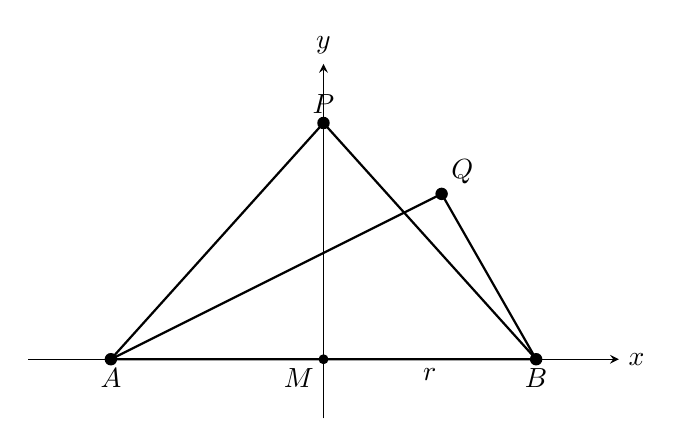
\begin{tikzpicture}[scale=1.5, >=stealth]
  \draw[->] (-2.5,0) -- (2.5,0) node[right] {$x$};
  \draw[->] (0,-0.5) -- (0,2.5) node[above] {$y$};
  
  \coordinate (M) at (0,0);
  \coordinate (A) at (-1.8,0);
  \coordinate (B) at (1.8,0);
  \coordinate (P) at (0,2.0);
  \coordinate (Q) at (1.0, 1.4);
  
  \draw[line width=0.8pt] (A) -- (P) -- (B) -- cycle;
  \draw[line width=0.8pt] (A) -- (Q) -- (B);
  
  \node[below left] at (M) {$M$};
  \node[below] at (A) {$A$};
  \node[below] at (B) {$B$};
  \node[above] at (P) {$P$};
  \node[above right] at (Q) {$Q$};
  
  \node[below] at (0.9,0) {$r$};
  
  \fill (M) circle (1.2pt);
  \fill (A) circle (1.5pt);
  \fill (B) circle (1.5pt);
  \fill (P) circle (1.5pt);
  \fill (Q) circle (1.5pt);
\end{tikzpicture}
\end{center}

\[
  Q\left(a \sin\left(\frac{\pi}{2}-\theta\right), a \cos\left(\frac{\pi}{2}-\theta\right)\right) = Q(a \sin\theta, a \cos\theta)
\]

\begin{enumerate}[(1)]
  \item $\tan \dfrac{\alpha}{2} = t$ とおくと $t = \dfrac{r}{a}$ だから
  \[
    \tan \alpha = \frac{2t}{1-t^2} = \frac{2(r/a)}{1-(r/a)^2} = \frac{2ra}{a^2-r^2}
  \]

  \item $\vec{QA} = \begin{pmatrix} -r - a \sin\theta \\ -a \cos\theta \end{pmatrix}$, $\vec{QB} = \begin{pmatrix} r - a \sin\theta \\ -a \cos\theta \end{pmatrix}$ から
  \begin{align*}
    \tan \beta &= \frac{|\vec{QA} \cdot \vec{QB} \cdot \sin\beta|}{\vec{QA} \cdot \vec{QB}} \\
    &= \frac{|(-r - a s)(-a c) - (r - a s)(-a c)|}{(r - a s)(-r - a s) + a^2 c^2} \quad (c = \cos\theta, s = \sin\theta) \\
    &= \frac{|2 r a c|}{a^2 - r^2} = \frac{2 r a c}{a^2 - r^2} \quad (\because 2 r a c > 0)
  \end{align*}
  だから
  \[
    \tan \alpha \cdot c = \frac{2 r a c}{a^2 - r^2} = \tan \beta
  \]
  である．
\end{enumerate}
\end{proof}

\newpage

\end{document}
